\section{\name{}} \label{sec:approach}
In this work, we treat model merging as combining the checkpoints (i.e., collection of weights) of multiple models into a single checkpoint that can perform all the tasks of its constituents. 
We do this by merging the layers of the models together.
For instance, suppose $L_i\in\mathcal{L}$ is a linear layer with parameters $W_i \in \mathbb{R}^{n_i\times m_i}, b_i \in \mathbb{R}^{n_i}$ with input features $x \in \mathbb{R}^{m_i}$ and outputs features $f_i \in \mathbb{R}^{n_i}$:
% For instance, if layer $L_i \in \mathcal{L}$ is a linear layer, it has parameters $W_i \in \mathbb{R}^{n_i\times m_i}, b_i \in \mathbb{R}^{n_i}$ and takes input $x \in \mathbb{R}^{m_i}$, with an output feature vector $f_i \in \mathbb{R}^{n_i}$ where
\begin{equation}\label{eq:linear_features}
    f_i = L_i(x) = W_i x + b_i
\end{equation}
Our goal is to take $\modela{L_i^A} \in \modela{\mathcal{L}^A}$ from \modela{model A} and $\modelb{L_i^B} \in \modelb{\mathcal{L}^B}$ from \modelb{model B} and merge them into a layer
% \footnote{Note that we consider activation and normalization to be distinct layers in the network as they are implemented in practice, rather than one combined unit.}
\modelc{$L_i^*$} that combines their feature spaces such that information from both \modela{$f_i^A$} and \modelb{$f_i^B$} is retained in \modelc{$f_i^*$}.
We accomplish this by merging each layer of one model with the corresponding layer in the other, both merging features in one \textit{across} both layers or \textit{within} the same layer.
% both \textit{within} and \textit{across} the layers: We merge each feature in one layer either to another feature either within the layer or across to another feature in the other layer. 
This is in contrast to permutation-based merging method, which only combine features \textit{across} layers.
% This is in-contrast to permutation-based merging, which only merges \textit{across} layers.
% We accomplish this by merging each layer of one model with the corresponding layer in the other, \textit{while modifying both} (in contrast to permutation-based merging, which only permutes one of the models).

\paragraph{Why should we merge \textit{within}?} % Because they solve different problems, features of models trained on different tasks may be dissimilar.
Features of models trained on different tasks may be dissimilar, as the models solve different problems. 
Forcibly combining these dissimilar features can yield merges that don't perform well on either original task (Fig~\ref{fig:loss_basin}).
Instead, those features may be more compatible with others within the same model, which would better retain performance when combined. % allowing them to be combined while retaining performance.
% These can be combined together and retain task capability.
% This can cause poor merges if they're combined with each other across the models. 
% However, these same features may be more similar (or redundant) to others \textit{within} the same model, making those better fits for merging.

In fact, we can \textit{prove} that methods which allow merges \textit{within} each model (as well as across both) perform equal to or \textit{better} than those which only merge across models (e.g., permutation-reliant approaches) in a limited but prevalent setting.
Specifically, we obtain a tighter bound over Theorem 3.1 from \citet{entezari2021role} when redundancy exists within a model and is leveraged. 
Both Theorem 3.1 and our Theorem \hyperref[ap:TheoremDef]{1} (see Appendix~\ref{ap:Theorem} for formalization and proof) bound the degree to which the loss of a merged two-layer model with $d$-input dimensions and $h$-intermediate dimensions increases compared to the losses of the original models. 
Theorem 3.1 bounds this increase to $\Tilde{O}(h^{-\sfrac{1}{(2d+4)}})$.
However, if features within a model are \textit{redundant}, then we reduce the bound to%
% (with $\Gamma\in[0,1]$ measuring what portion of features are redundant), then we substantially reduce the bound to
%is taken into account, then we substantially reduce the bound to,
%($0$ means nothing is similar and $1$ means everything is similar)
\begin{equation} \label{eq:mainpaper_barrier}
    \text{Loss Increase of Merged Model} \leq
        \begin{cases}
            \Tilde{O}\left(\left(\frac{h}{1-2\Gamma}\right)^{-\frac{1}{2d+4}}  \right) & \Gamma < 0.5 \\
            0 &\text{otherwise}
        \end{cases}
\end{equation}
with $\Gamma\in[0,1]$ measuring what portion of features are redundant. 
% This bound is 
This bound is %$\sqrt[2d+4]{1-2\Gamma} \leq 1$
$\sqrt[2d+4]{1-2\Gamma} \leq 1$
times that of Theorem 3.1 when $\Gamma < 0.5$ (equal only when $\Gamma = 0$) and \textit{explicitly zero} when $\Gamma \geq 0.5$.
% and is
% strictly less than Theorem 3.1 when $\Gamma\in(0,1]$ (achieving \textit{zero no matter $h$} when $\Gamma \geq 0.5$), and is only equal at $\Gamma=0$. 

% Prior work only modifies a single model \citep{ainsworth2022git,entezari2021role}. 
% These assume that features in one model have a similar counterpart in the second, and thus can be permuted from one model to match the second.
% However, the features of models trained on different tasks may be dissimilar because they solve different problems.
% In this case, no permutations may exist to match the two models.
% Instead, these features may be more similar (or redundant) to others in the same model and thus should be combined with those \textit{within} a model rather than \textit{across} models.

% We justify this intuition by \textbf{proving} that methods which exploit this phenomenon when it exists are \textit{strictly} better than permutation-reliant approaches in a limited but prevalent setting.
% Specifically, we obtain a significantly tighter bound over Theorem 3.1 from \citet{entezari2021role} in the same setting when similarity within a model exists and is leveraged.
% Theorem 3.1 bounds the degree to which permutations degrade the loss of a merged two-layer model with $d$-input dimensions and $h$-intermediate dimensions to $\Tilde{O}(h^{-\frac{1}{2d+4}})$.
% However, if we let $\Gamma$ denote the proportion of similar features within each model where $\Gamma\in[0,1]$, such that $\Gamma=0$ indicates nothing is similar and $\Gamma=1$ means everything is similar, we can leverage properties from \citet{simsek2021geometry} to obtain the tighter piece-wise bound:
% \begin{equation*}
%     \text{Loss Increase of Merged Model} \leq
%         \begin{cases}
%             \Tilde{O}\left(\left(\frac{h}{1-2\Gamma}\right)^{-\frac{1}{2d+4}}  \right) & \Gamma > 0.5 \\
%             0 &\text{otherwise}
%         \end{cases}
% \end{equation*}
% This bound is strictly lower than Theorem 3.1 when $\Gamma\in(0,1]$ with equality at $\Gamma=0$. 
% Also, unlike Theorem 3.1, it achieves zero-bound regardless of the intermediate dimension size when models have sufficient internal feature similarities. 
% Due to space restrictions, we leave further details and the proof to Appendix~\ref{ap:Theorem}.

% Please see Appendix~\ref{ap:Theorem} for more details. 

% In this work, we treat model merging as jointly combining the checkpoints (i.e., collection of weights) of two models into a single checkpoint that can perform all the tasks of its constituents.
% This is done by first transforming (e.g., prior work uses permutation) their and then interpolating between these new features in each model. 

% Models trained on different tasks solve different problems, causing their features to be more dissimilar.
% In this case, no permutation may exist to merge the models because some features in one model will not be similar to any in the second. 

% The features of models trained on different tasks 
% In this case, no permutation of features may

% When models are trained on different tasks, their features are far less likely to be similar 


% When models are trained on different tasks, their features become less correlated over the course of the network \citep{kornblith2019similarity}. 

% The features of models trained on different tasks become less correlated over the course of the network \citet{kornblith2019similarity}.
% In this case, no permutation of features may exist to merge the models and thus may permutation-based merging methods to fail.
% Instead, these divergent features between models should be processed via a method other than permutation.
% This makes permutation-based merging methods, which exactly map all features in one model to the other, substantially less likely to succeed.



% Permutation methods exactly map every feature in \modela{Model A} to \modelb{Model B} when merging them. 
% This inherently assumes that features across the models are similar, and more likely occurs when the models are trained on the same dataset. 
% However, the likelihood is much smaller when models are trained on different tasks, because their features become less correlated over the course of the network \citep{kornblith2019similarity}. 
% In this case\footnote{unless very rare conditions hold --- please see Appendix~\ref{ap:Theorem2_footnote}}, no permutation may exist to merge the models. 
% Instead, these divergent features between models should be processed via a method other than permutation.

% \paragraph{Merging Within Models.} 
% One way to address this problem is to exploit feature similarity \textit{within} \modela{Model A} and allows these features to be combined with others in \modela{Model A}, while permuting those similar \modelb{Model B} together.
% More specifically, this extends model merging by merging any combination of similar features \textit{within} models, and \textit{across} them.
% Notably, this supports many-1 and many-none in addition to 1-1 merging.
% First, it supports many-to-1 matching because any similar features within \modela{Model A} can be combined together before being permuted to their similar counterpart in \modelb{Model B}, and vice-versa.
% Second, it supports many-to-none matching because the same combined features may instead by matched to any empty feature in \modelb{Model B} obtained when its own features are merged.
% \name{} demonstrates the efficacy of \name{} through extensive empirical results---improving accuracy by up to \textbf{20\%} over permutation methods---and we further \textit{prove} its approach is \textbf{strictly} better than permutation methods under certain conditions---Appendix~\ref{ap:Theorem}. 

% In this work, we treat model merging as jointly combining the checkpoints (i.e., collection of weights) of two models into a single checkpoint that can perform all the tasks of its constituents. We accomplish this by merging each layer of one model with the corresponding layer in the other, \textit{while modifying both} (in contrast to permutation-based merging, which only permutes one of the models).

% For instance, if layer $L_i \in \mathcal{L}$ is a linear layer, it has parameters $W_i \in \mathbb{R}^{n_i\times m_i}, b_i \in \mathbb{R}^{n_i}$ and takes input $x \in \mathbb{R}^{m_i}$, with an output feature vector $f_i \in \mathbb{R}^{n_i}$ where
% \begin{equation}\label{eq:linear_features}
%     f_i = L_i(x) = W_i x + b_i
% \end{equation}
% Then our goal is to take $\modela{L_i^A} \in \modela{\mathcal{L}^A}$ from \modela{model A} and $\modelb{L_i^B} \in \modelb{\mathcal{L}^B}$ from \modelb{model B} and merge them into a layer \modelc{$L_i^*$} that combines their feature spaces such that information from both \modela{$f_i^A$} and \modelb{$f_i^B$} is retained in \modelc{$f_i^*$}.
% Note that we consider activation and normalization to be distinct layers in the network as they are implemented in practice, rather than one combined unit.



\paragraph{How do we merge features?}
% \paragraph{How do we obtain the combined features \modelc{$f_i^*$}?}
In prior work, each of the merged features \modelc{$f_i^*$} is the result of combining one feature from \modela{$f_i^A$} and one from \modelb{$f_i^B$}. 
However in our case, we can also merge features by combining two from just \modela{$f_i^A$} or two from just \modelb{$f_i^B$}. To account for this, we concatenate \modela{$f_i^A$} and \modelb{$f_i^B$} into a single feature vector:  $\modela{f_i^A}\|\modelb{f_i^B} \in \mathbb{R}^{2n_i}$. Then, like prior work (e.g. \citet{li2016convergenticlr,jordan2022repair}), we define feature similarity as the pairwise correlation between between neuron activations over a small set of images (without labels). However, unlike those works, we compute correlations between every activation in \textit{the full concatenated space} $\modela{f_i^A}\|\modelb{f_i^B}$. Our approach thus measures the similarity of every feature $\modela{f_i^A}$ and $\modelb{f_i^B}$ to all features in both models, rather than solely between $\modela{f_i^A}$ and $\modelb{f_i^B}$.
% If two features are very similar,
% then we can interpolate them without losing much information.
% These features can either be in $\modela{f_i^A}$ and $\modelb{f_i^B}$ (\textit{across} layers), or be in just $\modela{f_i^A}$ or $\modelb{f_i^B}$ (\textit{within} a layer).

% unlike permutation-based approaches (e.g. \citet{li2016convergenticlr,jordan2022repair}), we compute pairwise correlations between every neuron activation in \textit{the full concatenated space} $\modela{f_i^A}\|\modelb{f_i^B}$ over a small set of images (without labels).

Next, if two features are well correlated, we can average them without losing much information. Thus, we can construct \modelc{$f_i^*$} by finding $n_i$ pairs of similar features in $\modela{f_i^A}\|\modelb{f_i^B}$ and averaging them together. By default, we do this greedily: i.e., iteratively match the features with the highest correlation without replacement; though we explore extensions to this in Sec.~\ref{sec:extensions} and test other methods in Tab.~\ref{tab:matching_alg}. Then we can use these matches to construct \modelc{$f_i^*$}. Formally, we define a ``merge matrix'' $\modelc{M_i} \in \mathbb{R}^{n_i\times2n_i}$ s.t.
\begin{equation}
    \modelc{f_i^*} = \modelc{M_i}\left(\modela{f_i^A}\|\modelb{f_i^B}\right)
\end{equation}
$\modelc{M_i}$ averages the matched features, with each match corresponding to one output feature in $\modelc{f_i^*}$. For instance, if $u$th match is between indices $s, t \in \{1, \ldots, 2n_i\}$ of $\modela{f_i^A}\|\modelb{f_i^B}$, then the $u$th row of $\modelc{M_i}$ would be $\sfrac{1}{2}$ at columns $s$ and $t$ and 0 elsewhere. This results in $\modelc{f_i^*}[u] = \frac{1}{2} (\modela{f_i^A}\|\modelb{f_i^B})[s] + \frac{1}{2} (\modela{f_i^A}\|\modelb{f_i^B})[t]$.
Thus, applying $\modelc{M_i}$ has the effect of interpolating with $\gamma=\sfrac{1}{2}$ but is more general (e.g., allows for merging more than 2 models at once, see Sec.~\ref{sec:extensions}).

% We achieve this by first computing the pairwise correlations between every neuron activation in both \modela{$f_i^A$} and \modelb{$f_i^B$} over a label-less set of data.
% This differs from \citet{li2016convergenticlr,ainsworth2022git, entezari2021role, jordan2022repair} which instead only measure the pairwise correlation of neuron activations in $\modelb{f_i^B}$ to those in $\modela{f_i^A}$.
% As in prior work, we then define the similarity between any two features to simply be the correlation of the neuron activations from each.
% Notably, this means that our approach has the effect of measuring the similarity of every feature in either $\modela{f_i^A}$ and $\modelb{f_i^B}$ to all features in both models, rather than solely between $\modela{f_i^A}$ and $\modelb{f_i^B}$ as in prior work.

% We achieve this by first concatenating the feature vectors \modela{$f_i^A$} and \modelb{$f_i^B$} together into a vector:  $\modela{f_i^A}\|\modelb{f_i^B} \in \mathbb{R}^{2n_i}$.
% We then calculate the pairwise correlations of every feature in $\modela{f_i^A}\|\modelb{f_i^B}$ with every other feature in the vector---following the strategy of \citep{li2016convergenticlr}.
% This has the effect of measuring the correlation of every feature in either $\modela{f_i^A}$ and $\modelb{f_i^B}$ to all features in both models.
% Note, this differs from \citet{li2016convergenticlr,ainsworth2022git, entezari2021role, jordan2022repair} which instead only measure the correlation of features in $\modelb{f_i^B}$ to those in $\modela{f_i^A}$.
% If two features are highly correlated, 
% If two features are very similar,
% then we can interpolate them without losing much information.
% These features can either be in $\modela{f_i^A}$ and $\modelb{f_i^B}$ (\textit{across} layers), or be in just $\modela{f_i^A}$ or $\modelb{f_i^B}$ (\textit{within} a layer).

% \textcolor{red}{
% Thus, if we can find a good pairing for each element in both $\modela{f_i^A}$ and $\modelb{f_i^B}$ (leaving us with $n_i$ pairs), we can construct a merged feature \modelc{$f_i^*$} that contains an efficiently compressed representation of $\modela{f_i^A}$ and $\modelb{f_i^B}$ by averaging each pair of features. 
% This is equivalent to interpolating with $\gamma=\sfrac{1}{2}$.
% In practice we apply this merge in two steps. First, we concatenate the feature vectors \modela{$f_i^A$} and \modelb{$f_i^B$} together into a vector:  $\modela{f_i^A}\|\modelb{f_i^B} \in \mathbb{R}^{2n_i}$.
% Second, we define a ``merge matrix'' $\modelc{M_i} \in \mathbb{R}^{n_i\times2n_i}$ such that
% }
% Thus, if we can find a good pairing for each element of the concatenated $\modela{f_i^A}\|\modelb{f_i^B}$ (leaving us with $n_i$ pairs), we can construct a merged feature \modelc{$f_i^*$} that contains an efficiently compressed representation of $\modela{f_i^A}$ and $\modelb{f_i^B}$ by 
% averaging each pair of features. 
% \textcolor{red}{This is equivalent to interpolating with $\gamma=\sfrac{1}{2}$.}
% % \textcolor{red}{interpolating each pair of features}.
% In practice, we apply this merge by defining a ``merge matrix'' $\modelc{M_i} \in \mathbb{R}^{n_i\times2n_i}$ such that
% \begin{equation}
%     \modelc{f_i^*} = \modelc{M_i}\left(\modela{f_i^A}\|\modelb{f_i^B}\right)
% \end{equation}
% % The resulting \modelc{$M_i$} is non-zero (taking a value of $\sfrac{1}{2}$ only at indices corresponding to feature pairs in $\modela{f_i^A}\|\modelb{f_i^B}$ that are merged together.
% The resulting \modelc{$M_i$} is $\sfrac{1}{2}$ for indices corresponding to matched pairs in $\modela{f_i^A}\|\modelb{f_i^B}$ and 0 elsewhere. Thus, \modelc{$M_i$} has the effect of selects paired features from $\modela{f_i^A}\|\modelb{f_i^B}$ and averaging them.
% % is zero everywhere except for each pair with index $p$ of matches $(j, k)$, \modelc{${M_i}_{[p,j]} = {M_i}_{[p,k]} = \sfrac{1}{2}$}. 
% We find these matches greedily---an optimal algorithm exists but is very slow and only slightly more accurate (Tab.~\ref{tab:matching_alg}).


% In order to construct the combined features \modelc{$f_i^*$}, we assume that there are some redundant features in \modela{$f_i^A$} and \modelb{$f_i^B$}. 
% That is, we assume some elements of the two feature vectors are \textit{highly correlated} over a sample of data. 
% \textcolor{blue}{
% We use the same definition of correlation as in \citep{li2016convergenticlr}.
% }
% In this work, we consider correlations between features \textit{within} the same model and \textit{across} the two models. In practice we concatenate the two feature vectors into $\modela{f_i^A}\|\modelb{f_i^B} \in \mathbb{R}^{2n_i}$ and consider correlations between each pair of elements in this concatenated vector, which differs from prior work \cite{ainsworth2022git,jordan2022repair} that only consider correlations \textit{across} the two models.

% If two features are highly correlated, then we can average them without losing much information.
% Thus, if we can find a good pairing for each element of the concatenated $\modela{f_i^A}\|\modelb{f_i^B}$ (leaving us with $n_i$ pairs), we can construct a merged feature \modelc{$f_i^*$} that contains an efficiently compressed representation of $\modela{f_i^A}$ and $\modelb{f_i^B}$ by averaging each pair of features. In practice, we define a merge matrix $\modelc{M_i} \in \mathbb{R}^{n_i\times2n_i}$ s.t.
% \begin{equation}
%     \modelc{f_i^*} = \modelc{M_i}\left(\modela{f_i^A}\|\modelb{f_i^B}\right)
% \end{equation}
% The resulting \modelc{$M_i$} is zero everywhere except for each pair with index $p$ of matches $(j, k)$, \modelc{${M_i}_{[p,j]} = {M_i}_{[p,k]} = \sfrac{1}{2}$}. We find these matches greedily---an optimal algorithm exists but is very slow and only slightly more accurate (Tab.~\ref{tab:matching_alg}).


\paragraph{What about the next layer?}
After merging features in one layer, we now have the problem that the next layers, $\modela{L_{i+1}^A}, \modelb{L_{i+1}^B}$, are incompatible with $\modelc{f_i^*}$. Instead, we need to \textit{undo} the merge operation before passing the features to the next layer. Thus, we define an ``unmerge'' matrix $\modelc{U_i} \in \mathbb{R}^{2n_i \times n_i}$ s.t.
\begin{equation}
    \modelc{U_i f_i^*} \approx \modela{f_i^A}\|\modelb{f_i^B}
\end{equation}
$\modelc{U_i}$ is the pseudoinverse of $M_i$ and in the case of the matching from earlier is simply $2\modelc{M_i}^T$.
% In the case of the matching from earlier, $\modelc{U_i}$ has the effect of ``copying'' the merged features back to their original locations and is simply $2\modelc{M_i}^T$ (with $2\times$ to cancel out the $\sfrac{1}{2}$ from averaging).
% In the case of the matching from earlier, $\modelc{U_i}$ is simply $2\modelc{M_i}^T$ and has the effect of ``copying'' the merged features back to their original locations. 
%Note that in most cases, we can't have a strict equality here because $\modelc{U_i}$ isn't full rank.
Note that strict equality is unlikely here. Like in prior work, merging models is a lossy operation. % , we can't have a strict equality here because $\modelc{U_i}$ isn't full rank.

We 
% can further 
split this unmerge matrix in half along its rows into $\modela{U_i^A}, \modelb{U_i^B} \in \mathbb{R}^{n_i\times n_i}$ that act individually to produce \modela{$f_i^A$} and \modelb{$f_i^B$}. 
% by splitting \modelc{$U_i$}  in half along its rows. 
With this, we can evaluate the next layers using the merged features:
\begin{equation}
    \modela{f_{i+1}^A} \approx \modela{L_{i+1}^A}(\modela{U_i^A} \modelc{f_i^*}) \qquad \modelb{f_{i+1}^B} \approx \modelb{L_{i+1}^B}(\modelb{U_i^B} \modelc{f_i^*})
\end{equation}



\subsection{The ``Zip'' Operation}
We now have
% Now that we have
all 
the necessary pieces, 
% we 
and can derive a general operation to merge \modela{$L_i^A$} and \modelb{$L_i^B$} at an arbitrary point in the network (Fig.~\ref{fig:zip_op}).
First, we compute \modelc{$M_i$} and \modelc{$U_i$} by matching features between \modela{$f_i^A$} and \modelb{$f_i^B$}. We then pass \modelc{$U_i$} to the next layer and receive \modelc{$U_{i-1}$} from the previous layer. Using \modelc{$M_i$} and \modelc{$U_{i-1}$}, we 
% can now 
``fuse'' the merge and unmerge operations into the layer's parameters. For a linear layer:
\begin{equation} \label{eq:zip}
    % \modelc{W^*_i} = \gamma\modela{M_i^A W_i^A U^A_{i-1}} + (1-\gamma)\modelb{M_i^B W_i^B U^B_{i-1}}
    \modelc{W^*_i} = \modela{M_i^A W_i^A U^A_{i-1}} + \modelb{M_i^B W_i^B U^B_{i-1}}
\end{equation}
where \modela{$M_i^A$} and \modelb{$M_i^B$} are \modelc{$M_i$} split along its columns.
% and $\gamma$ is a hyperparameter we set to $\sfrac{1}{2}$.
\modelc{$b_i^*$} has the same equation but without unmerging.

Note the similarity between Eq.~\ref{eq:zip} and Eq.~\ref{eq:rebasin}. This isn't a coincidence: if we only allowed merging \textit{across} models and not \textit{within} models, our ``zip'' operation would be identical to Git Re-Basin's permute-then-interpolate approach. Thus, Eq.~\ref{eq:zip} can be thought of as a generalization of prior work.


\begin{figure*}
    \centering
    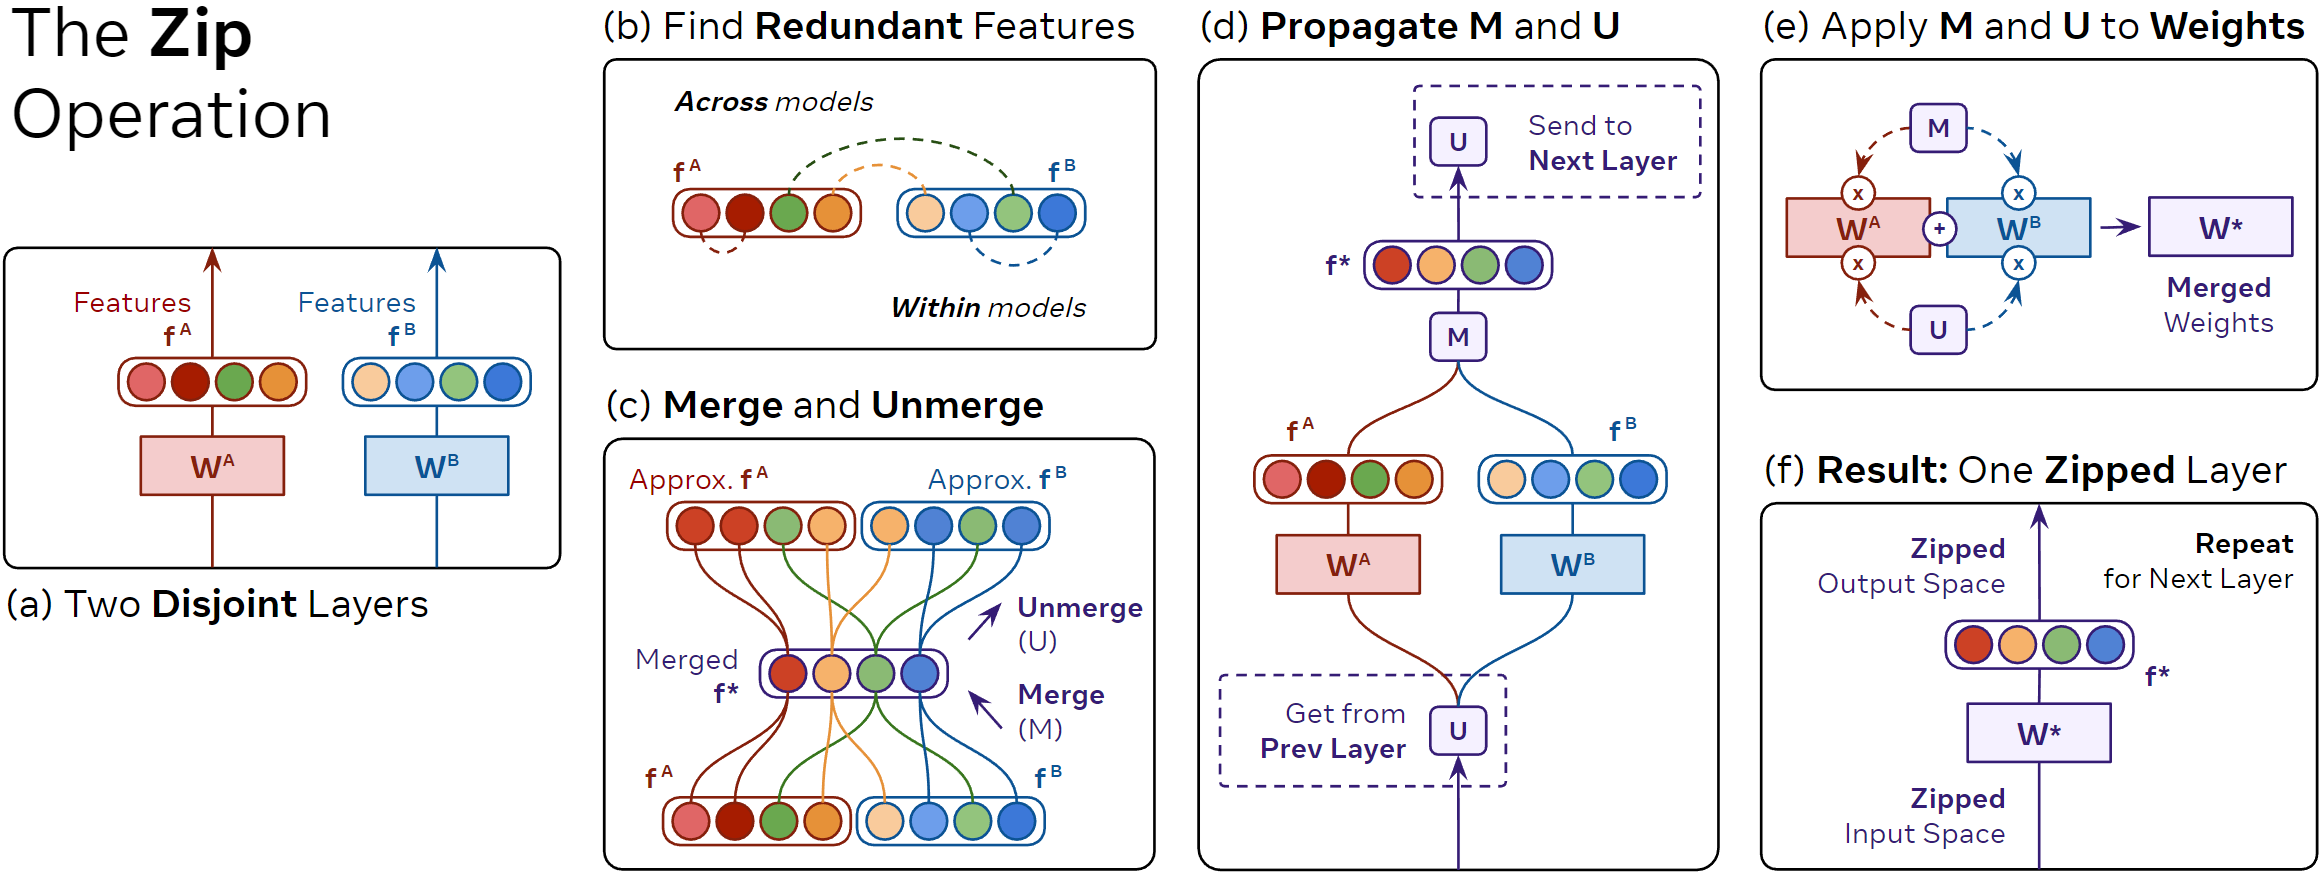
\includegraphics[width=0.95\linewidth]{figures/imgs/zip_it.png}
    \caption{{\bf \name{}} merges models layer-wise by exploiting redundancy in their features. 
    % (a) Starting with completely disjoint layers with weights \modela{$W^{A}$} and \modelb{$W^{B}$} from models trained on different tasks, (b) we match redundant features by comparing their activations \modela{$f^{A}$} and \modelb{$f^{B}$}. (c) We use this matching to produce a merge matrix \modelc{M} to combine \modela{$f^{A}$} and \modelb{$f^{B}$} into a single shared feature space \modelc{$f^{*}$} and a corresponding unmerge matrix \modelc{U} that undoes this operation. (d) In order to align the input space of the next layer, we propagate \modelc{U} forward along network and at the same time receive a \modelc{U} matrix from the previous layer. (e) Once we have both an \modelc{M} for the output, and a \modelc{U} for the input, we can ``zip'' the layers together by applying Eq.~\ref{eq:zip}. (f) The result is a single layer with a shared input and output space, and we can now repeat from (a) on the next layer.
    (a) Output features \modela{$f^{A}$} and \modelb{$f^{B}$} from two disjoint layers are (b) paired with other features based on the similarity of their activations. (c) We produce a merge matrix \modelc{M} to combine the pairs into a single shared output feature space, and a corresponding unmerge matrix \modelc{U} that undoes this operation. (d) We then propagate \modelc{U} up the network to align the next layer's input space, and simultaneously receive the previous layer's \modelc{U} to align our input space. (e) We apply Eq.~\ref{eq:zip} to ``zip'' the layers together using the \modelc{M} for the output and \modelc{U} for the input, producing a single layer (f). We then repeat (a) on the next layer.
    % . (f) We obtain a single layer with a shared input and output space. We then repeat from (a) on the next layer. 
    }
    \label{fig:zip_op}
\end{figure*}
\begin{figure}[t]
\centering

\begin{minipage}{0.48\linewidth}{
    \centering
    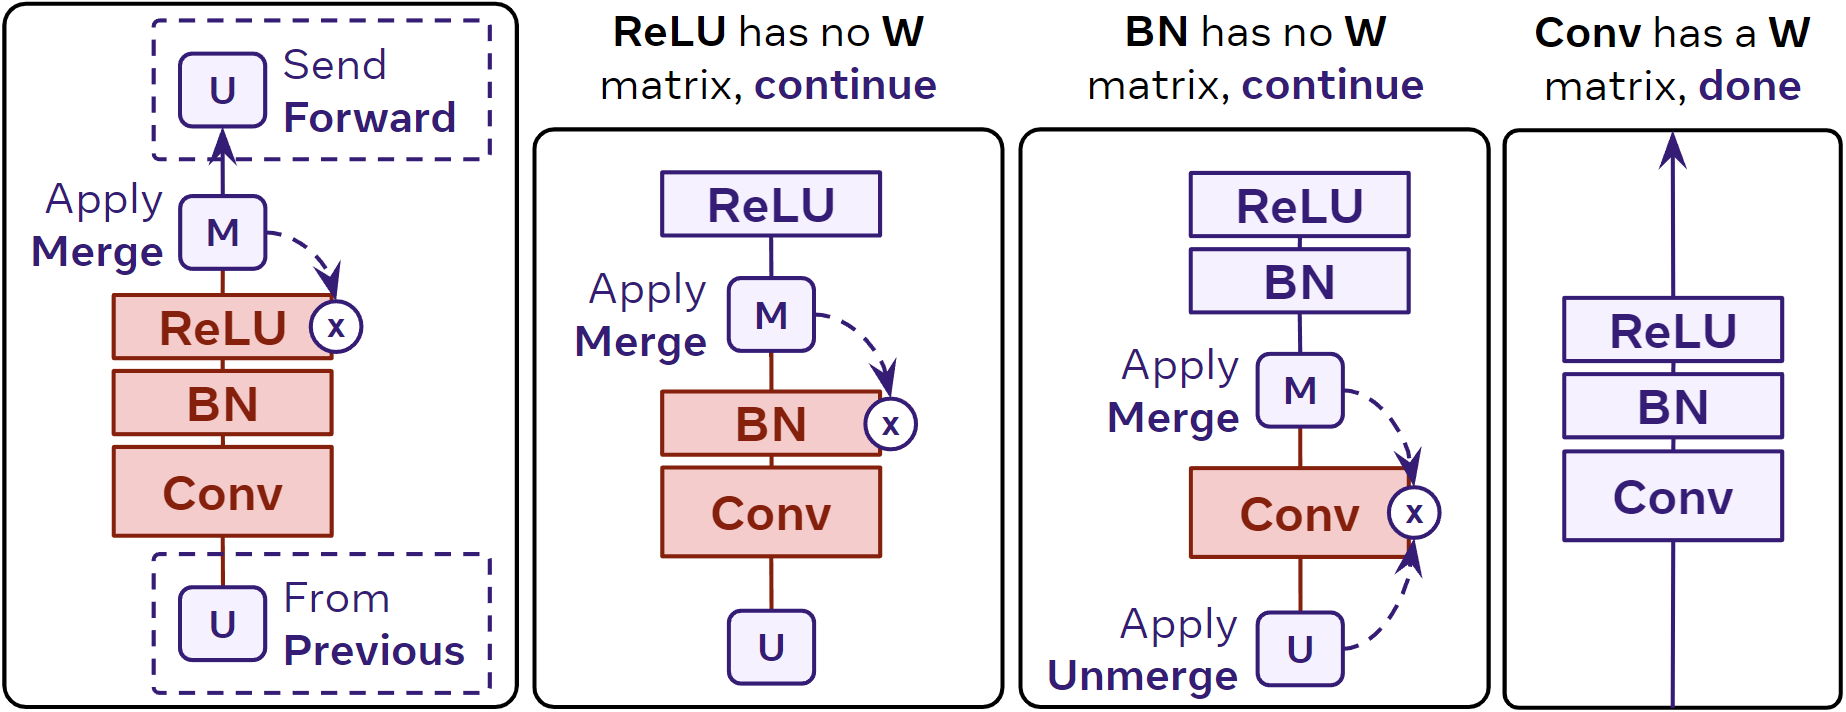
\includegraphics[width=\linewidth]{figures/imgs/zip_prop.png}
    \caption{{\bf Zip Propagation.} 
    % In practice, we compute \modelc{$M_i$} and \modelc{$U_i$} after activations (e.g., ReLU). 
    We propagate \modelc{$M_i$} backward until we hit a layer with weights, merging merging element-wise layers (e.g., BatchNorm) along the way.
    % We can't apply Eq.~\ref{eq:zip} to a layer without a weight matrix and have to propagate \modelc{$M_i$} backward until we hit such a layer. all element-wise layers (e.g., BatchNorm) are merged along the way.
    % Since we can't apply Eq.~\ref{eq:zip} to a layer without a weight matrix, we have to propagate \modelc{$M_i$} backward until we hit such a layer, merging element-wise layers (e.g., BatchNorm) along the way.
    }
    \label{fig:zip_prop}
}\end{minipage}
\hspace{1em}
\begin{minipage}{0.48\linewidth}{
    \centering
    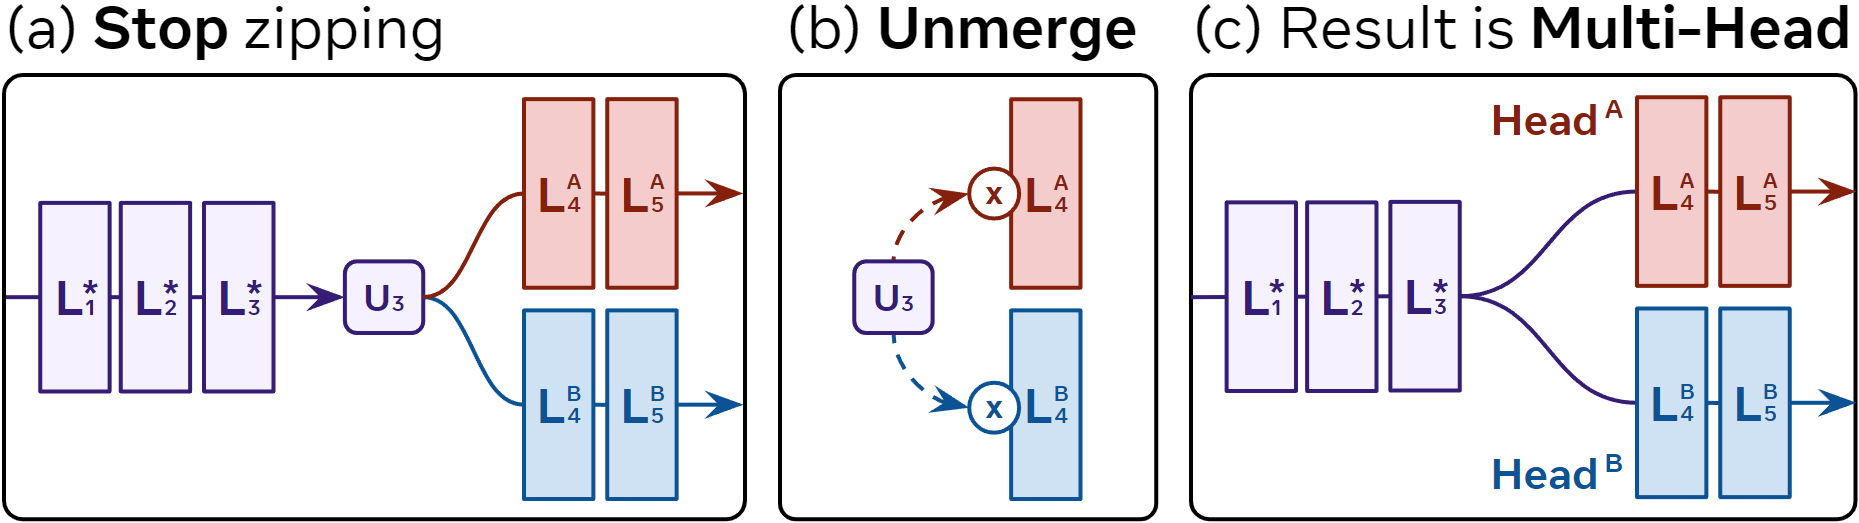
\includegraphics[width=\linewidth]{figures/imgs/partial_zip.png}
    \caption{
        {\bf Partial Zip.}
        (a) If we stop zipping early and (b) apply the latest \modelc{U} from the zip propagation to the inputs of the first unmerged layer in each model, (c) we get a multi-head model with a head for each task.
        % If we stop zipping early (a), we can create a multi-head model that can perform multiple tasks. All we need to do is apply the last unmerge from zip propogation (Fig.~\ref{fig:zip_prop}) to the inputs of the first unmerged layer in each model (b), and we get a model with multiple heads (c).
    }
    \label{fig:partial_zip}
}\end{minipage}
\vspace{-10pt}
\end{figure}

\subsection{Zip Propagation} \label{sec:zip_prop}
However, most modern neural networks are not simply collections of linear layers stacked on top of each other. In practice, we cannot combine merge and unmerge matrices into every layer of the network, as a local zip (Eq.~\ref{eq:zip}) expects the layer to have a weight \textit{matrix}---i.e., the layer has to have separate input and output spaces so that we can unmerge the input space and merge the output space. Other layers (e.g., BatchNorm, ReLU) don't have such a weight matrix.

Thus, we ``propogate'' \modelc{$M_i$} and \modelc{$U_i$} \textit{through} these layers. For instance, in Fig.~\ref{fig:zip_prop}, we show a common stack of layers found in a typical ConvNet. Following \citet{jordan2022repair}, we compute \modelc{$M_i$} and \modelc{$U_i$} using the activations of the network (i.e., after each ReLU). We can't fuse \modelc{$M_i$} with the ReLU layer, as it doesn't have any parameters. Similarly, we can merge the parameters of the preceding BatchNorm layer (i.e., in the same way as bias). But it doesn't have a weight matrix, so we also can't fuse \modelc{$M_i$} into it. Only once we've reached the Conv layer can we fuse \modelc{$M_i$} and \modelc{$U_i$} into it using Eq.~\ref{eq:zip} (in this case, treating each kernel element as independent).

Similar care needs to be taken with skip connections, as every layer that takes input from or outputs to a skip connection shares the same feature space. However, this too can be dealt with during propagation---we just need to propagate \modelc{$M_i$} backward and \modelc{$U_i$} forward to each layer connected by the same skip connection. 
In general, we can define propagation rules to handle many different types of network modules (see Appendix~\ref{ap:prop_rules}).


\subsection{Extensions}\label{sec:extensions}

\paragraph{Partial Zip.} \label{sec:partial_zip}
% In many cases, 
We don't always want to zip every layer of the two networks, especially if their output spaces are incompatible, or if doing so would lose too much accuracy. 
% In those cases, 
Instead, we can perform a \textit{partial zip}. That is, we zip most of the layers together, but leave
% some of 
the later ones \textit{unzipped} (Fig.~\ref{fig:partial_zip}).

Implementing this operation is simple in our framework: zip as normal until the specified layer $i$, then the remaining unzipped layers will receive \modelc{$U_i$} through zip propagation. If we apply \modela{$U_i^A$} to \modela{$L_{i+1}^A$} and \modelb{$U_i^B$} to \modelb{$L_{i+1}^B$}, the remaining unzipped layers will form ``heads'' that expect merged features as input. We can then ensemble the heads or choose one to evaluate at runtime.

\paragraph{Repeated Matching ($\alpha$).} In some cases, we'd like to merge more than two models together. To do this, we allow ``repeated matches''. That is, when two features are matched in our greedy algorithm, they are removed and replaced with the resulting merged feature. To ensure that one feature doesn't get merged endlessly, we set the correlations of the new feature to be the minimum of the old features' similarities weighted by $\alpha \in (0,1]$. We find a small value of $\alpha$ typically works best.

\paragraph{Same-model Budget ($\beta$).} To demonstrate the effectiveness of same-model merges, we introduce a ``budget'' parameter $\beta \in [0, 1]$ that denotes what percent of total merged features can come from models merging within themselves, with each model receiving an equal portion of this budget. Note that a budget of 0 results in Eq.~\ref{eq:rebasin}, as in that case no features can be merged within models.
